\documentclass[./../../paper.tex]{subfiles}
\graphicspath{{\subfix{./../../figures/}}}

\begin{document}

We cannot use the \gls{damerau_levenshtein} for process mining, if the process carries additional information about event attributes. Mainly, because two events may be emitted by the same activity, but they may still carry different event attributes. 

% TODO: Change a, b and c to x, y and z or e_1, e_2 and e_3
To illustrate the issue, we explore a couple of examples. Lets assume, we have two strings $s^1=aaba$ and $s^2=acba$. Using the \gls{damerau_levenshtein}, the edit distance between both sequences is 1, as we can recognise a substitution at the second position in both strings. However, this representation is insufficient for process instances. Therefore, we now characterise the two sequences as process events rather than strings in \autoref{eq:dlexample}. 

\begin{align}
    \label{eq:dlexample}
    s^1 &=\{a,a,b,a\} \\
    s^2 &=\{a,a^*,b,a\}\\
    s^3 &=\{a,c,b,a\}\\
    s^4 &=\{a,a,b\}
    &a,b,c \in \mathbb{R}^3\\
    a &= \begin{bmatrix}
        2\\
        1\\
        4\\
    \end{bmatrix}
    a^* = \begin{bmatrix}
        3\\
        3\\
        4\\
    \end{bmatrix}
    b = \begin{bmatrix}
        1\\
        1\\
        0\\
    \end{bmatrix}
    c = \begin{bmatrix}
        3\\
        1\\
        4\\
    \end{bmatrix}
\end{align}

\noindent If we do not consider attribute values, it becomes clear that $s^2$, $s^3$ and $s^4$ have an edit-distance to $s^1$ of 0, 1 and 1. However, with attribute values in mind, $s^1$ and $s^2$ display clear differences. Similarly, $s^1$ and $s^3$ not only differ in terms of activity but also attribute value. Lastly, $s^1$ and $s^4$ are the same in attribute values, but one element still misses entirely. These examples show that we can neither disregard attribute values nor events, while computing the edit distance of two \glspl{instance}. 
We show this in \autoref{fig:image_with_dl}. 
In other words, we cannot simply assume a static cost of 1 for each edit operation. Instead, we have to define a cost function which takes attribute variables into account. In the following sections, we will establish distances which use a modified \gls{damerau_levenshtein} approach. Here, the cost of each edit-operation will be weighted with a distance function that considers the difference between event attributes. In simplified terms, we can say that $s^1$ and $s^2$ are identical, if we only consider the activity. However, taking attribute values into account, $s^1$ and $s^2$ actually differ on two accounts. 

% \begin{figure}[htb]
%     \centering
%     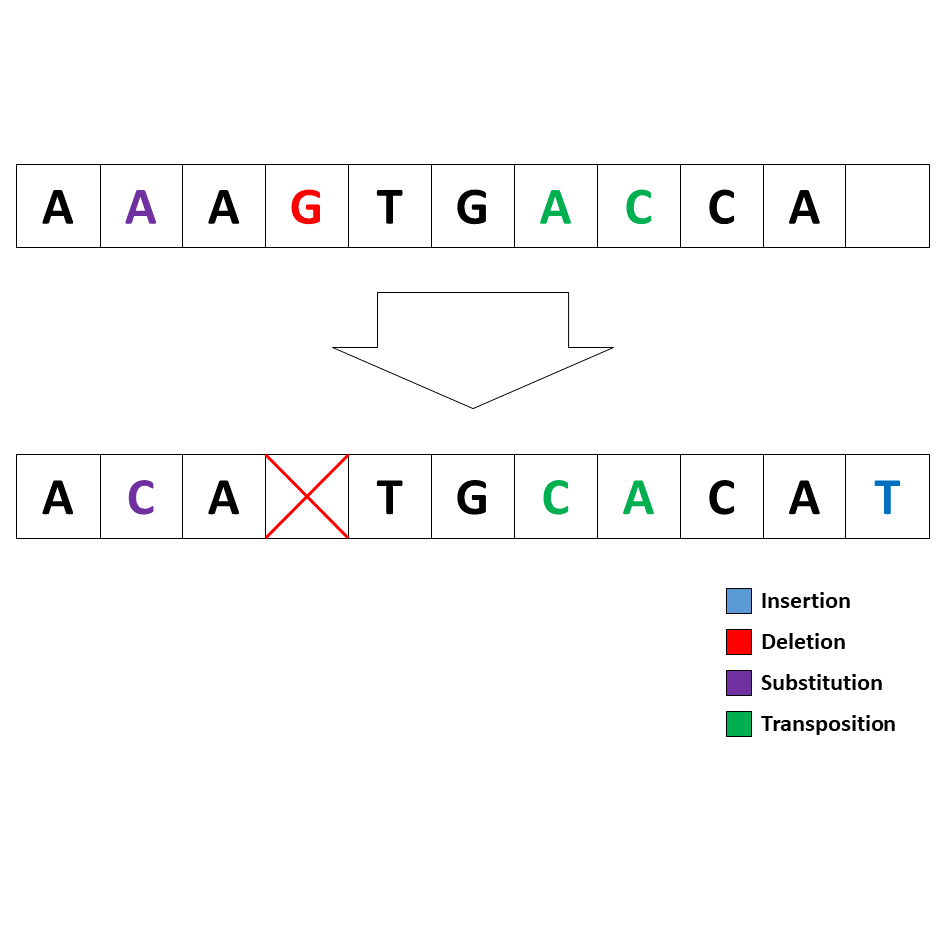
\includegraphics[width=0.99\textwidth]{figures/Graphics/Slide6.PNG}
%     \caption{This figure exemplifies the differeneces between the normal DL-distance and this one used.}
%     \label{fig:image_with_dl}
% \end{figure}

% \needsfigure{fig:image_with_dl}{This figure exemplifies the differeneces between the normal DL-distance and this one used.}

\noindent In order to reflect these differences in attribute values, we introduce a modified version of the \gls{damerau_levenshtein}, that not only reflects the difference between two process instances, but also the attribute values. We achieve this by introducing a cost function $\editCost$, which applies to a normed vector-space\footnotemark. Concretely, we formulate the modified \gls{damerau_levenshtein} as shown in \autoref{eq:modified_dl}. For the remainder, we will denote this edit-distance as \gls{SSDLD}.\footnotetext{A normed vector-space is a vector space, in which all vectors have the same dimensionality. For instance, if all vectors have three dimensions, we can call the vector-space \emph{normed}.}
% TODO: Introduce a with a dash above to compare activities instead of the vector
% Make zero thicker to indicate a null vector
\begin{align}
    \label{eq:modified_dl}
    d_{a, b}(i, j) & =\min
    \begin{cases}
        \editDistance{i-1}{j  }+\editCostFunctionNoA & \text { if } i>0                                            \\
        \editDistance{i  }{j-1}+\editCostFunctionNoB & \text { if } j>0                                            \\
        \editDistance{i-1}{j-1}+\editCostFunctionBoth & \text { if } i, j>0   \\ & \text { \& } \overline{a}_i=\overline{b}_j                                       \\
        \editDistance{i-1}{j-1}+ \editCostFunctionNoB +\editCostFunctionNoA  & \text { if } i, j>0  \\ & \text { \& } \overline{a}_i \neq \overline{b}_j                                       \\
        \editDistance{i-2}{j-2}+\editCostFunction{a_i}{b_{j-1}} + \editCostFunction{a_{i-1}}{b_j} & \text { if } i, j>1 \\ 
        & \text { \& } \overline{a}_i=\overline{b}_{j-1} \\ 
        & \text { \& } \overline{a}_{i-1}=\overline{b}_j \\
        0                                 & \text { \& } i=j=0                                          
    \end{cases} 
\end{align}

\noindent Here, $d_{a, b}(i, j)$ is the recursive form of the Damerau-Levenshtein-Distance. $a$ and $b$ are sequences and $i$ and $j$ specific elements of the sequence. $cost(a,b)$ is a cost function which takes the attribute values of $a$ and $b$ into account. 
The first two terms correspond to a deletion and an insertion from $a$ to $b$. The idea is to compute the maximal cost for that the wrongfully deleted or inserted event. 
The third term adds the difference between two events with identical activities $\overline{a}_i$ and $\overline{b}_j$. As mentioned earlier, two events that refer to the same activity can still be different due to event attributes. The distance between the event attributes determines \emph{how} different these events are. 
The fourth term handles the substitution of two events. Here, we compute the substitution cost as the sum of an insertion and a deletion. 
The fifth term computes the cost after transposing both events. This cost is similar to term 3 only that we now consider the differences between both events after they were aligned. The last term relates to the stopping criterion of the recursive formulation of the \gls{damerau_levenshtein}.  


\end{document}